\section{Entwurfsmuster}

Nach dem Architekten Christopher Alexander lässt sich ein Entwurfsmuster folgendermaßen beschreiben:\\
\\

\blockquote{Each pattern describes a problem which occurs over and over again in our environment, and then describes the core of the solution to that problem, in such a way that you can use this solution a million times over, without ever doing it the same way twice.}\footnote{dt.: Jedes Muster beschreibt ein Problem, das in unserer Umgebung immer wieder auftritt und beschreibt dann den Kern der Lösung für dieses Problem, und zwar so, dass Sie diese Lösung millionenfach anwenden können, ohne sie jemals zweimal auf die gleiche Weise zu verwirklichen.} \cite{gamma_design_1995}\\
\\

Obwohl diese Aussage auf Gebäude bezogen war, lässt sie sich ebenso gut auch Softwarearchitekturen anwenden. Auch in der Planung großer Softwaresysteme treten häufig dieselben abstrakten Probleme auf, welche sich mit einer Menge von Entwurfsmusters lösen lassen, welche die Beziehungen und Interaktionen von Objekten spezifizieren.

Ein Entwurfsmuster besteht dabei immer aus vier Elementen, seinem Namen, einer Problembeschreibung, einer Lösung und den sich ergebenden Konsequenzen \cite{gamma_design_1995}. Die Problembeschreibung gibt dabei an, in welchen Fällen sich ein Muster anwenden lässt, während die Lösung die Beziehungen und Verantwortlichkeiten der beteiligten Objekte beschreibt. Sie geht dabei nicht auf individuelle Anwendungsfälle ein, sondern stellt lediglich eine abstrakte Herangehensweise an das Problem bereit. Jedes Muster bringt Vor- und Nachteile mit sich und geht Kompromisse zwischen verschiedenen Qualitätsaspekten ein. Die Konsequenzen beleuchten diese und helfen bei der Argumentation für oder gegen eine konkrete Designentscheidung.

Im Folgenden werden die abstrakten Entwurfsmusters beschrieben, welche in der Architekturdiskussion eine Rolle spielen werden.

\subsection{Strategy Pattern}
\subsection{Template Method}

\subsubsection*{Problembeschreibung}

Es existieren ein Algorithmus, welcher aus einer Menge von Teilschritten besteht. Die einzelnen Teilschritte sollen austauschbar gehalten werden, um ein flexibles Anpassen des Algorithmus zu ermöglichen. Die Reihenfolge der Teilschritte ist hingegen festgelegt. 

\subsubsection*{Lösung}

\begin{figure}[!hb]
	\centering
	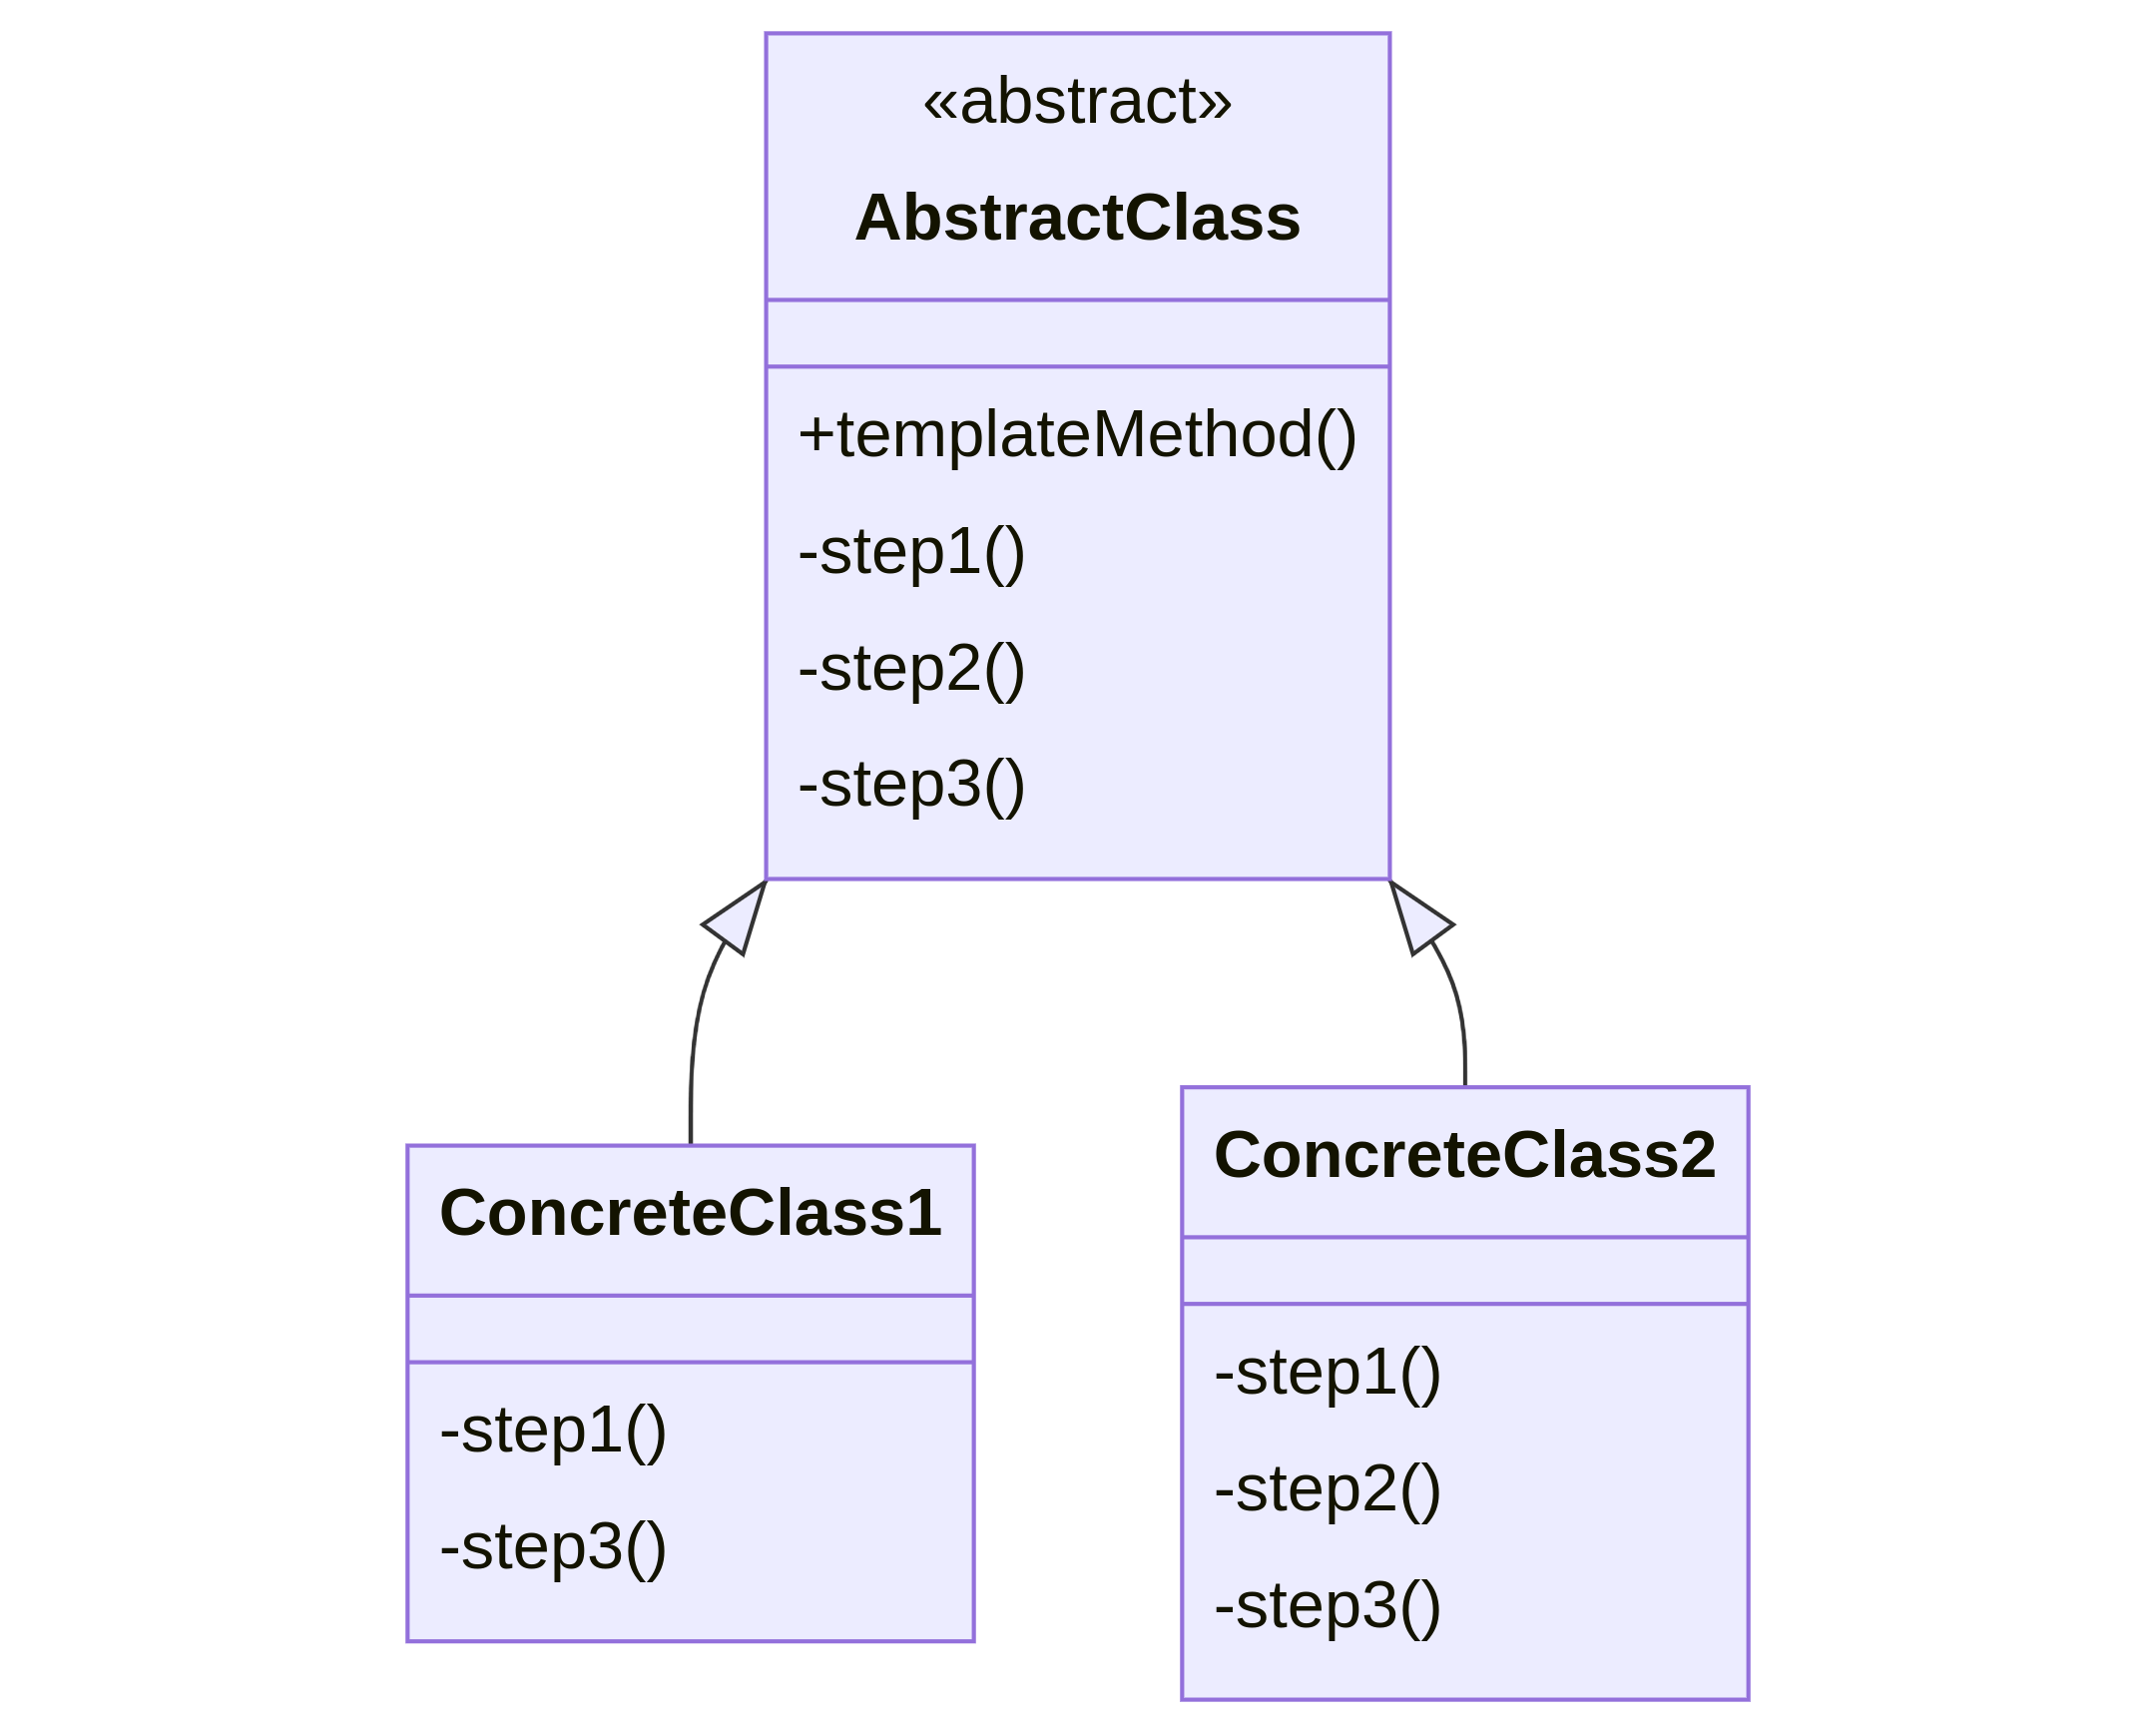
\includegraphics[width=0.75\linewidth]{images/patterns/template-method-class.png}
	\caption{Klassendiagramm Template Method}
	\label{fig:template-method-class}
\end{figure}

Jede Klasse, welche einen Algorithmus der selben Struktur implementiert, erbt von einer abstrakten Klassen, welche die `templateMethod` implementiert. Diese gibt das Grundgerüst des Algorithmus vor und ruft darin die einzelnen Teilschritte auf. Diese sind jeweils in eigenen Methoden implementiert. Die Subklassen definieren diese Methoden zum Teil neu, wenn eine Veränderung des Verhaltens dieses Teilschrittes notwendig ist.


\lstset{language=python}
\begin{lstlisting}[caption={Quelltextunterschrift}, label=code:template-method-code]
class AbstractClass:
	def templateMethod(self):
    	if self.step1():
        	self.step2()
    	self.step3()
\end{lstlisting}


\subsubsection*{Konsequenzen}

Template Methods sind ein Mechanismus, welcher die Wiederverwendung von Code ermöglicht und kann somit der Codeduplikation entgegen wirken. Anstatt Abwandlungen von Algorithmen von Grund auf neu zu implementieren, ist es möglich, sie aus bestehenden Komponenten zusammenzusetzen und je nach Bedarf neuen Code hinzuzufügen. Das Muster der Template-Method weist eine umgekehrte Kontrollstruktur auf. Anstatt dass eine Klasse Methoden ihrer Superklasse aufruft, delegiert die Template-Method die Verantwortlichkeit für die einzelnen Teile des Algorithmus an sie Subklassen.

Bei der Verwendung der Template-Method ist jedoch zu beachten, wie die einzelnen Methoden zu verwenden sind. Diese lassen sich grob in zwei Arten einteilen, Die "Hook"-Methoden und die abstrakten Methoden. Während die "Hook"-Methoden eine Standard-Implementierung in der abstrakten Basisklasse bereitstellen, ist dies bei den abstrakten Methoden nicht der Fall. Entsprechend müssen die abstrakten Methoden zwingend von einer konkreten Subklasse implementiert werden. Bei den "Hook"-Methoden ist das optional. 

Die Template-Method synergiert mit dem Strategy-Pattern. Einzelne Schritte eine Algorithmus können in einer Strategie-Klasse implementiert sein.
\subsection{Observer Pattern}


\subsubsection*{Problembeschreibung}

Häufig müssen verschiedene Komponenten eines Systems synchron gehalten werden. Gleichzeitig soll aber auch eine enge Kopplung dieser Komponenten vermieden werden. Es wird eine $1$:$n$-Beziehung zwischen den Objekten benötigt, wobei $n$ Objekte von einem Objekt abhängen. Wenn das eine Objekt seinen Zustand ändert, so sollen alle abhängigen Objekte benachrichtigt werden, sodass auch sie ihren Zustand aktualisieren können. Ein naiver Lösungsansatz wäre, jedem abhängigen Objekt eine Referenz auf das Objekt zu geben, von welchem es abhängt. Die Objekte könnten dann in regelmäßigen Abständen prüfen, ob eine Zustandsänderung stattgefunden hat (\emph{Polling}). Dieser Ansatz weist jedoch nicht nur eine hohe Kopplung auf, er ist auch wenig performant. Auch wenn keine Zustandsänderung stattgefunden hat, wird auf diese geprüft. Der Aufwand für diese Prüfung steigt dabei linear mit der Anzahl der beteiligten Objekte.

Das \emph{Observer-Pattern} kann Anwendung finden, wenn es zwei voneinander getrennte Konzepte gibt und eines von dem anderen abhängig ist. Die Abhängigkeit kann modelliert werden, ohne die Objekte stark zu koppeln. Weiterhin ist es möglich, die Anzahl der abhängigen Objekte variablen zu halten. \cite{gamma_design_1995}

\subsubsection*{Lösung}

Das Observer-Pattern besteht aus einem Sender (\code{Publisher}) und mehreren Empfängern (\code{ConcreteSubscriber}). Die Empfänger implementieren die Empfänger-Schnittstelle (\code{Subscriber}), welches eine Methode \code{update} zur Aktualisierung des Zustandes bereitstellt. Der Sender hält eine Liste von Referenzen auf Empfänger und verfügt über die Methoden \code{subscribe} und \code{unsubscribe}, welche es ermöglichen, der Liste Empfänger hinzuzufügen, oder sie zu entfernen (siehe Abbildung \ref{fig:observer-class}).

\begin{figure}[htb]
	\centering
	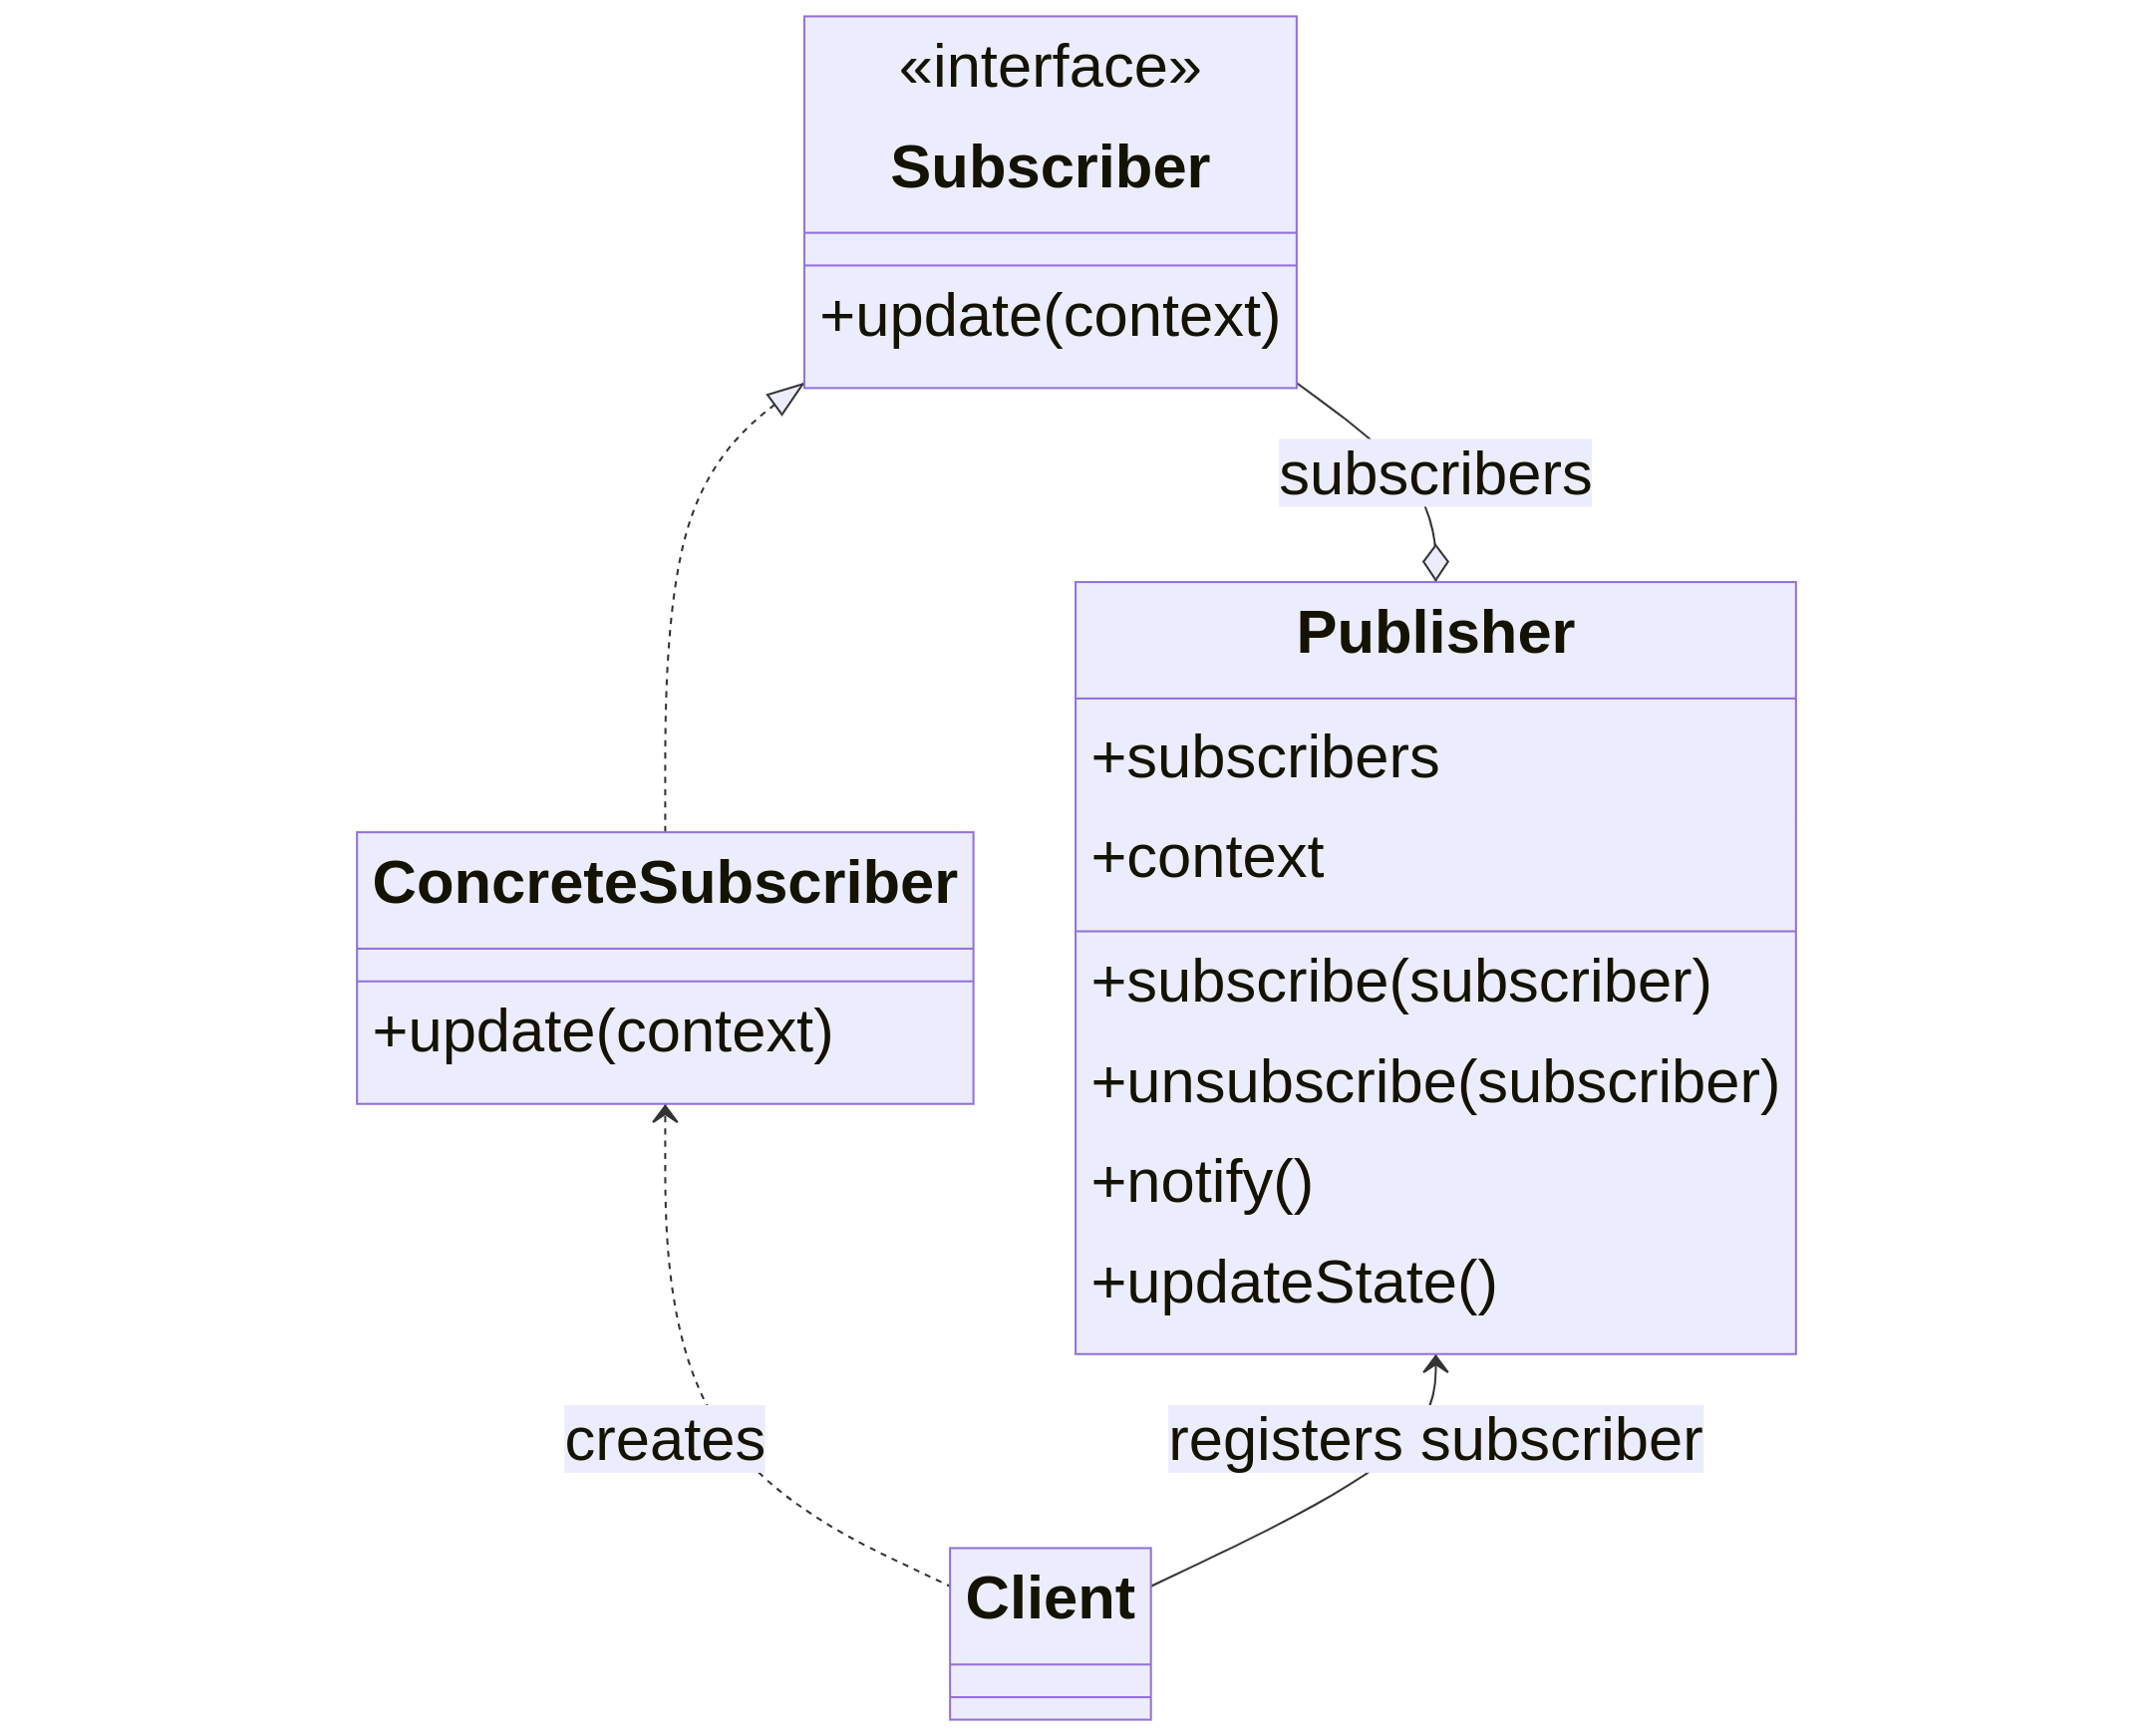
\includegraphics[width=0.95\linewidth]{images/patterns/observer-class.png}
	\caption{Klassendiagramm des Observer-Patterns \cite{skobeleva_observer_2023}}
	\label{fig:observer-class}
\end{figure}

Abbildung \ref{fig:observer-seq} zeigt, dass der Anwender (\code{Client})\footnote{Der Anwender (\code{Client}) ist in der Regel eine weitere Klasse, welche den beschriebenen Mechanismus verwendet. Es handelt sich in aller Regel nicht um einen Meenschen.} den Zustand des Sender durch Senden von \code{updateSate} verändern kann (1). Der Sender sendet sich draufhin selbst \code{notify} (2) und beginnt über seine Liste von Empfängern zu iterieren. Jedem Empfänger sendet er dann \code{update} (3, 5) und übergibt den notwendigen Kontext, sodass der Empfänger seinen Zustand entsprechend aktualisieren kann.

\begin{figure}[htb]
	\centering
	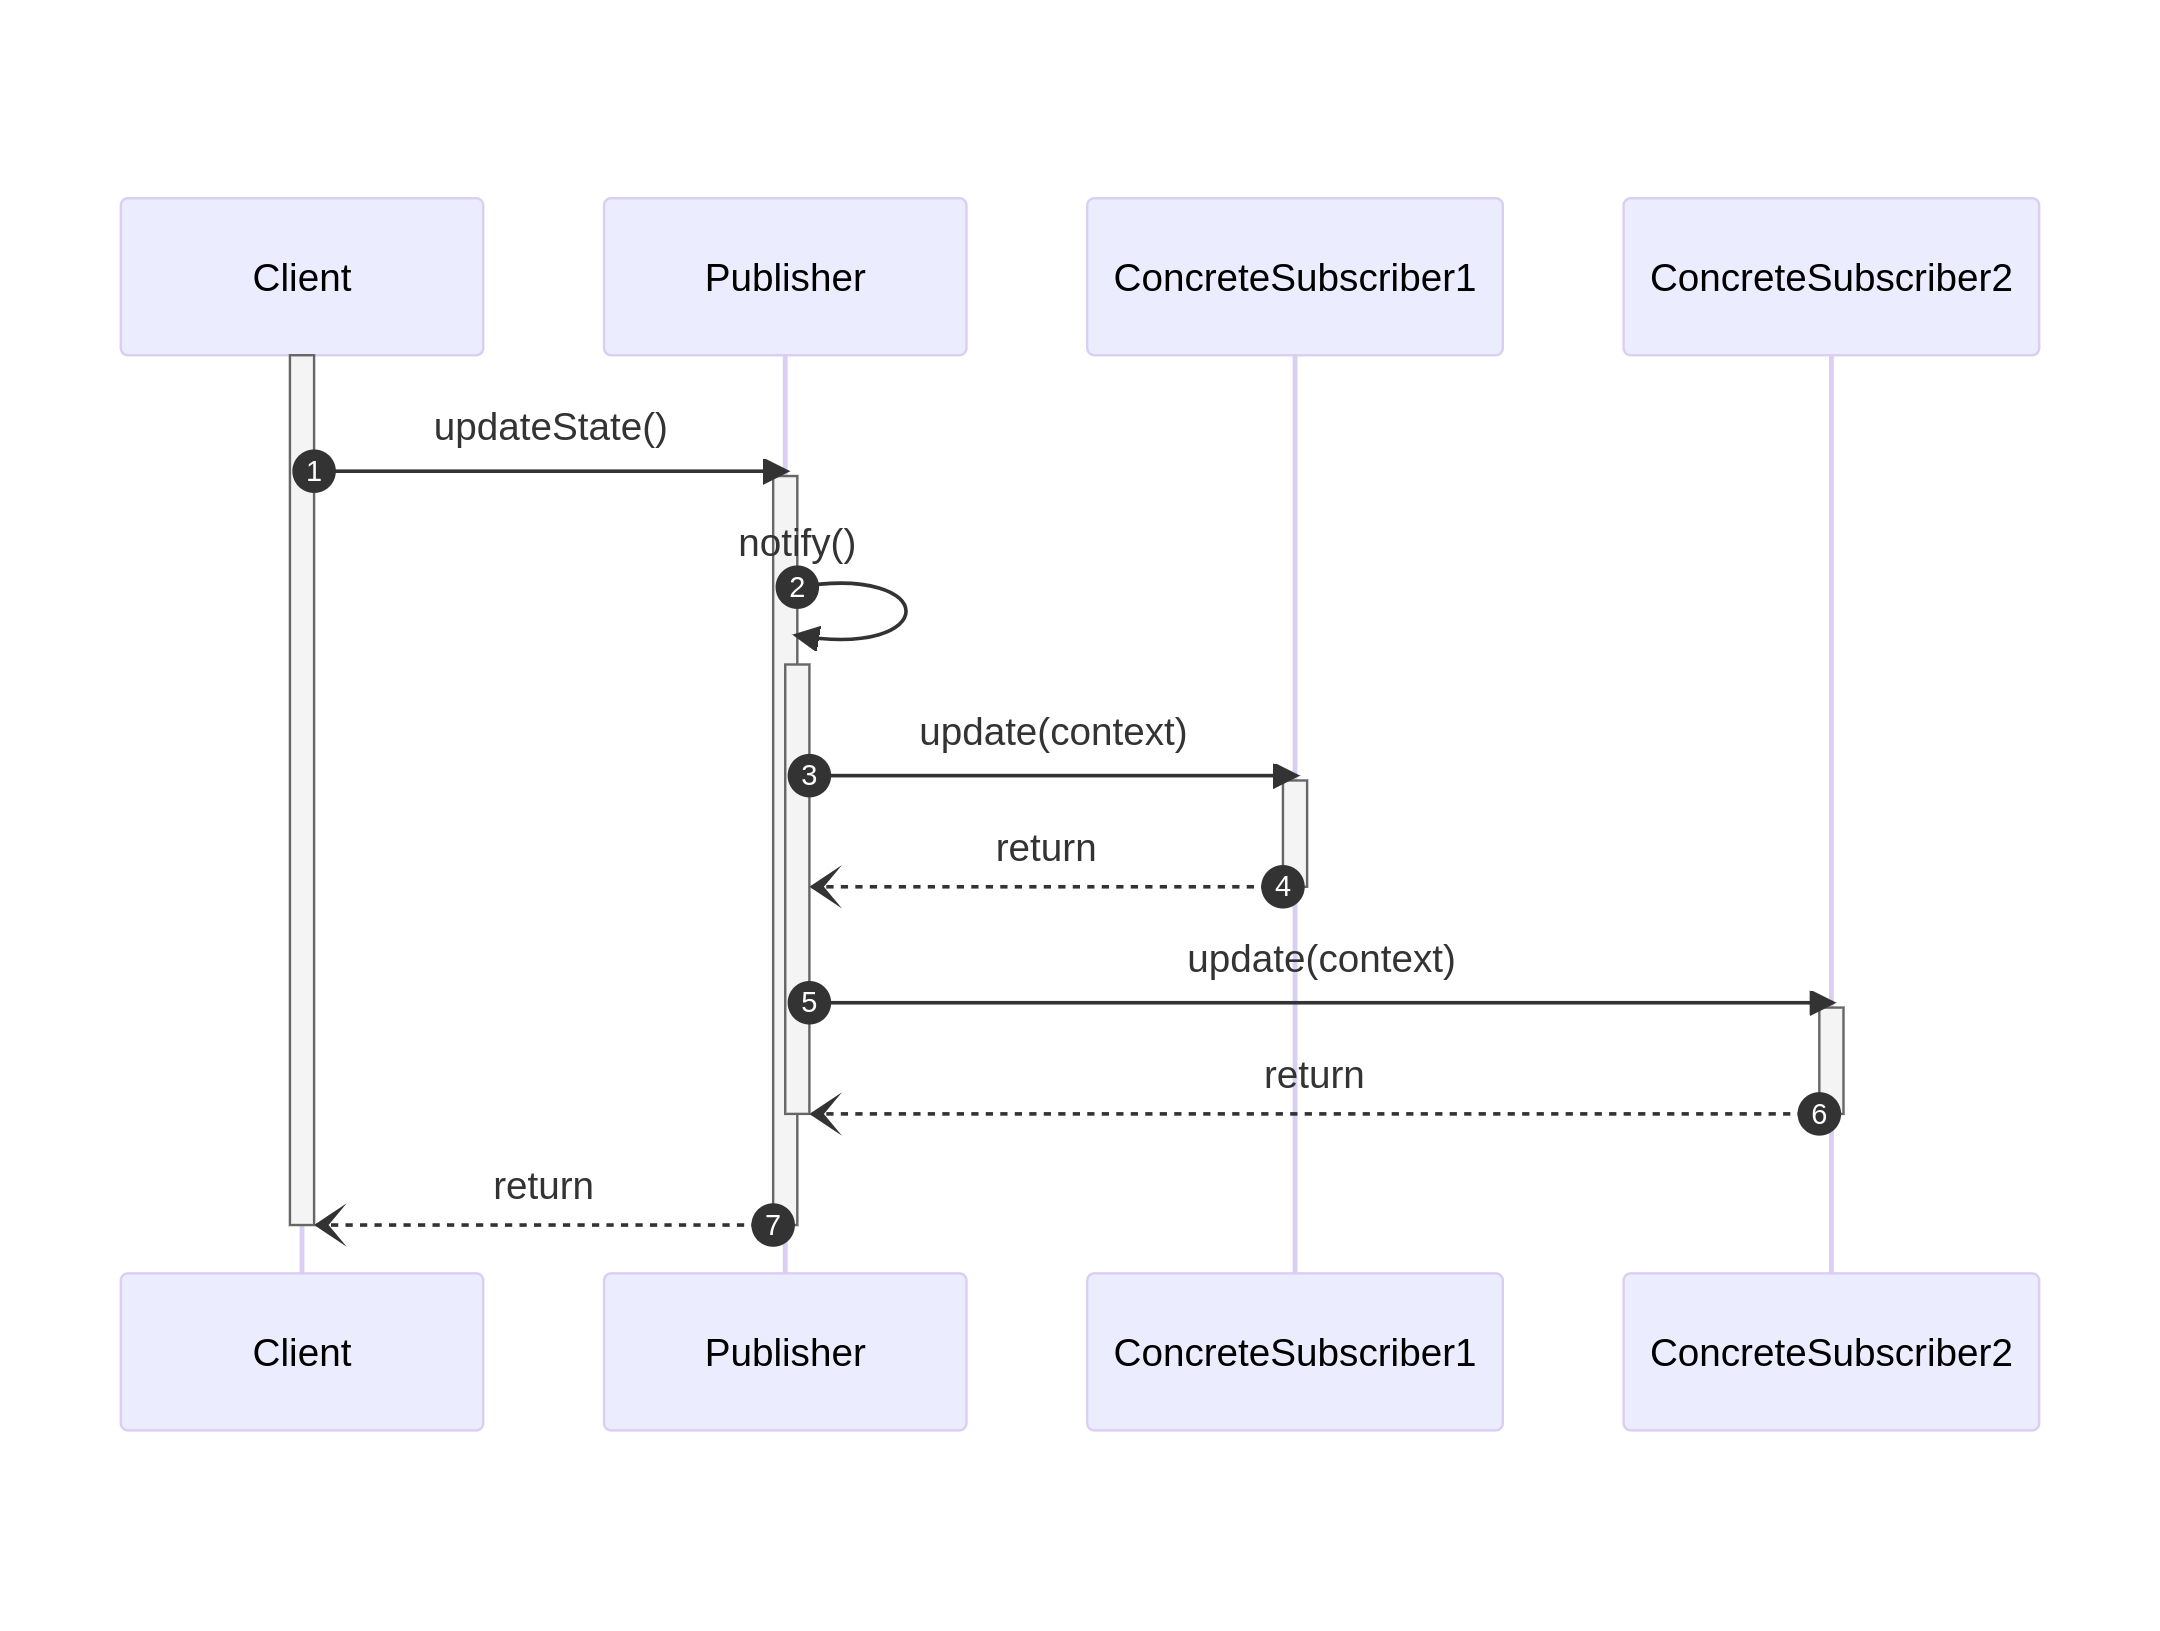
\includegraphics[width=0.95\linewidth]{images/patterns/observer-seq.png}
	\caption{Sequenzdiagramm des Observer-Patterns \cite{skobeleva_observer_2023}}
	\label{fig:observer-seq}
\end{figure}

Quelltext \ref{code:observer-code} veranschaulicht die Benachrichtigung aller Empfänger. In \code{notify} wird an jeden im Sender referenzierten Empfänger \code{update} gesendet. Dabei wird der Kontext des Senders an jeden Empfänger übergeben.

\lstset{language=python}
\begin{lstlisting}[caption={Quelltext der Methode \code{notify} des Publishers, welche über alle Empfänger iteriert und diese benachrichtigt.}, label=code:observer-code]
class Publisher
	def notify(self):
        for subscriber in self.subscribers:
            subscriber.update(self.context)
\end{lstlisting}


\subsubsection*{Konsequenzen}

Das Observer-Pattern bietet eine Reihe von Vorteilen. Durch Separation von Sender und Empfänger und durch die Abstraktion der Empfänger-Schnittstelle wird eine lose Kopplung der beiden erreicht. Diese lose Kopplung ermöglicht es, sowohl den Sender, als auch die Empfänger beliebig auszutauschen. Weiterhin können sich der Sender und die Empfänger auf unterschiedlichen Abstraktionsniveaus befinden. Ein Sender auf einem niedrigen Level kann einen Empfänger auf einem hohen Level benachrichtigen. Wären Empfänger und Sender nicht getrennt, so wäre dafür ein Abstraktionshierarchie-übergreifendes Objekt notwendig, welches die Trennung der Abstraktionsschichten beeinträchtigen würde. Ein weiterer Vorteil ist die dynamische Anzahl der Empfänger, mit denen ein Sender interagieren kann. So kann der Anwender über den Sender eine beliebige Zahl an Empfängern erreichen.

Ein Nachteil des Observer-Patterns ist, dass der Sender stets alle seine Empfänger benachrichtigt. Es kann vorkommen, dass nur eine Teilmenge der Empfänger die Benachrichtigung benötigt, was in unnötigen Methodenaufrufen resultiert. \cite{gamma_design_1995}
\subsection{Mediator Pattern}


\subsubsection*{Problembeschreibung}

Große Softwareprojekte bestehen meist aus einer einer enormen Anzahl an Klassen bzw. Objekten, welche miteinander interagieren. Ziel ist es stets, die Kopplung zwischen diesen Komponenten so gering wie möglich zu halten. Komplexe Interaktionsmuster zwischen diesen Objekten lassen sich nicht immer verhindern, das sie die inhärente Komplexität des modellierten Problems wiederspiegeln. In diesem Fall ist eine Lösung notwending, die diese Komplexität kapselt. Das Mediator-Pattern ist in der Lage, solche Fälle von komplexer Interaktion zu vereinfachen.

\subsubsection*{Lösung}

Der konkrete Mediator implementiert das Mediator-Interface, welches eine Methode `notify` bereitstellt, um Benachrichtigungen der einzelnen Komponenten entgegenzunehmen. Jede Komponente besitzt eine Referenz auf den Mediator, um `notify`an ihn senden zu können. Dabei übergibt die Komponente sich selbst, um dem Mediator den Kontext der Benachrichtigung bereitzustellen. In Abhängigkeit des übergebenen Senders und dessen Zustand, führt der Mediator eine (komplexe) Logik aus, welche vollständig innerhalb des Mediators gekapselt ist. Der Mediator hält ebenso Referenzen auf alle Komponenten, die er zu beeinflussen in der Lage sein soll. Die gekapselte Logik kann somit die Interfaces der Komponenten verwenden, um diese zu beeinflussen. Dadurch findet eine indirekte Beeinflussung von Komponenten durch andere Komponenten über den Mediator statt.  

\begin{figure}[!hb]
	\centering
	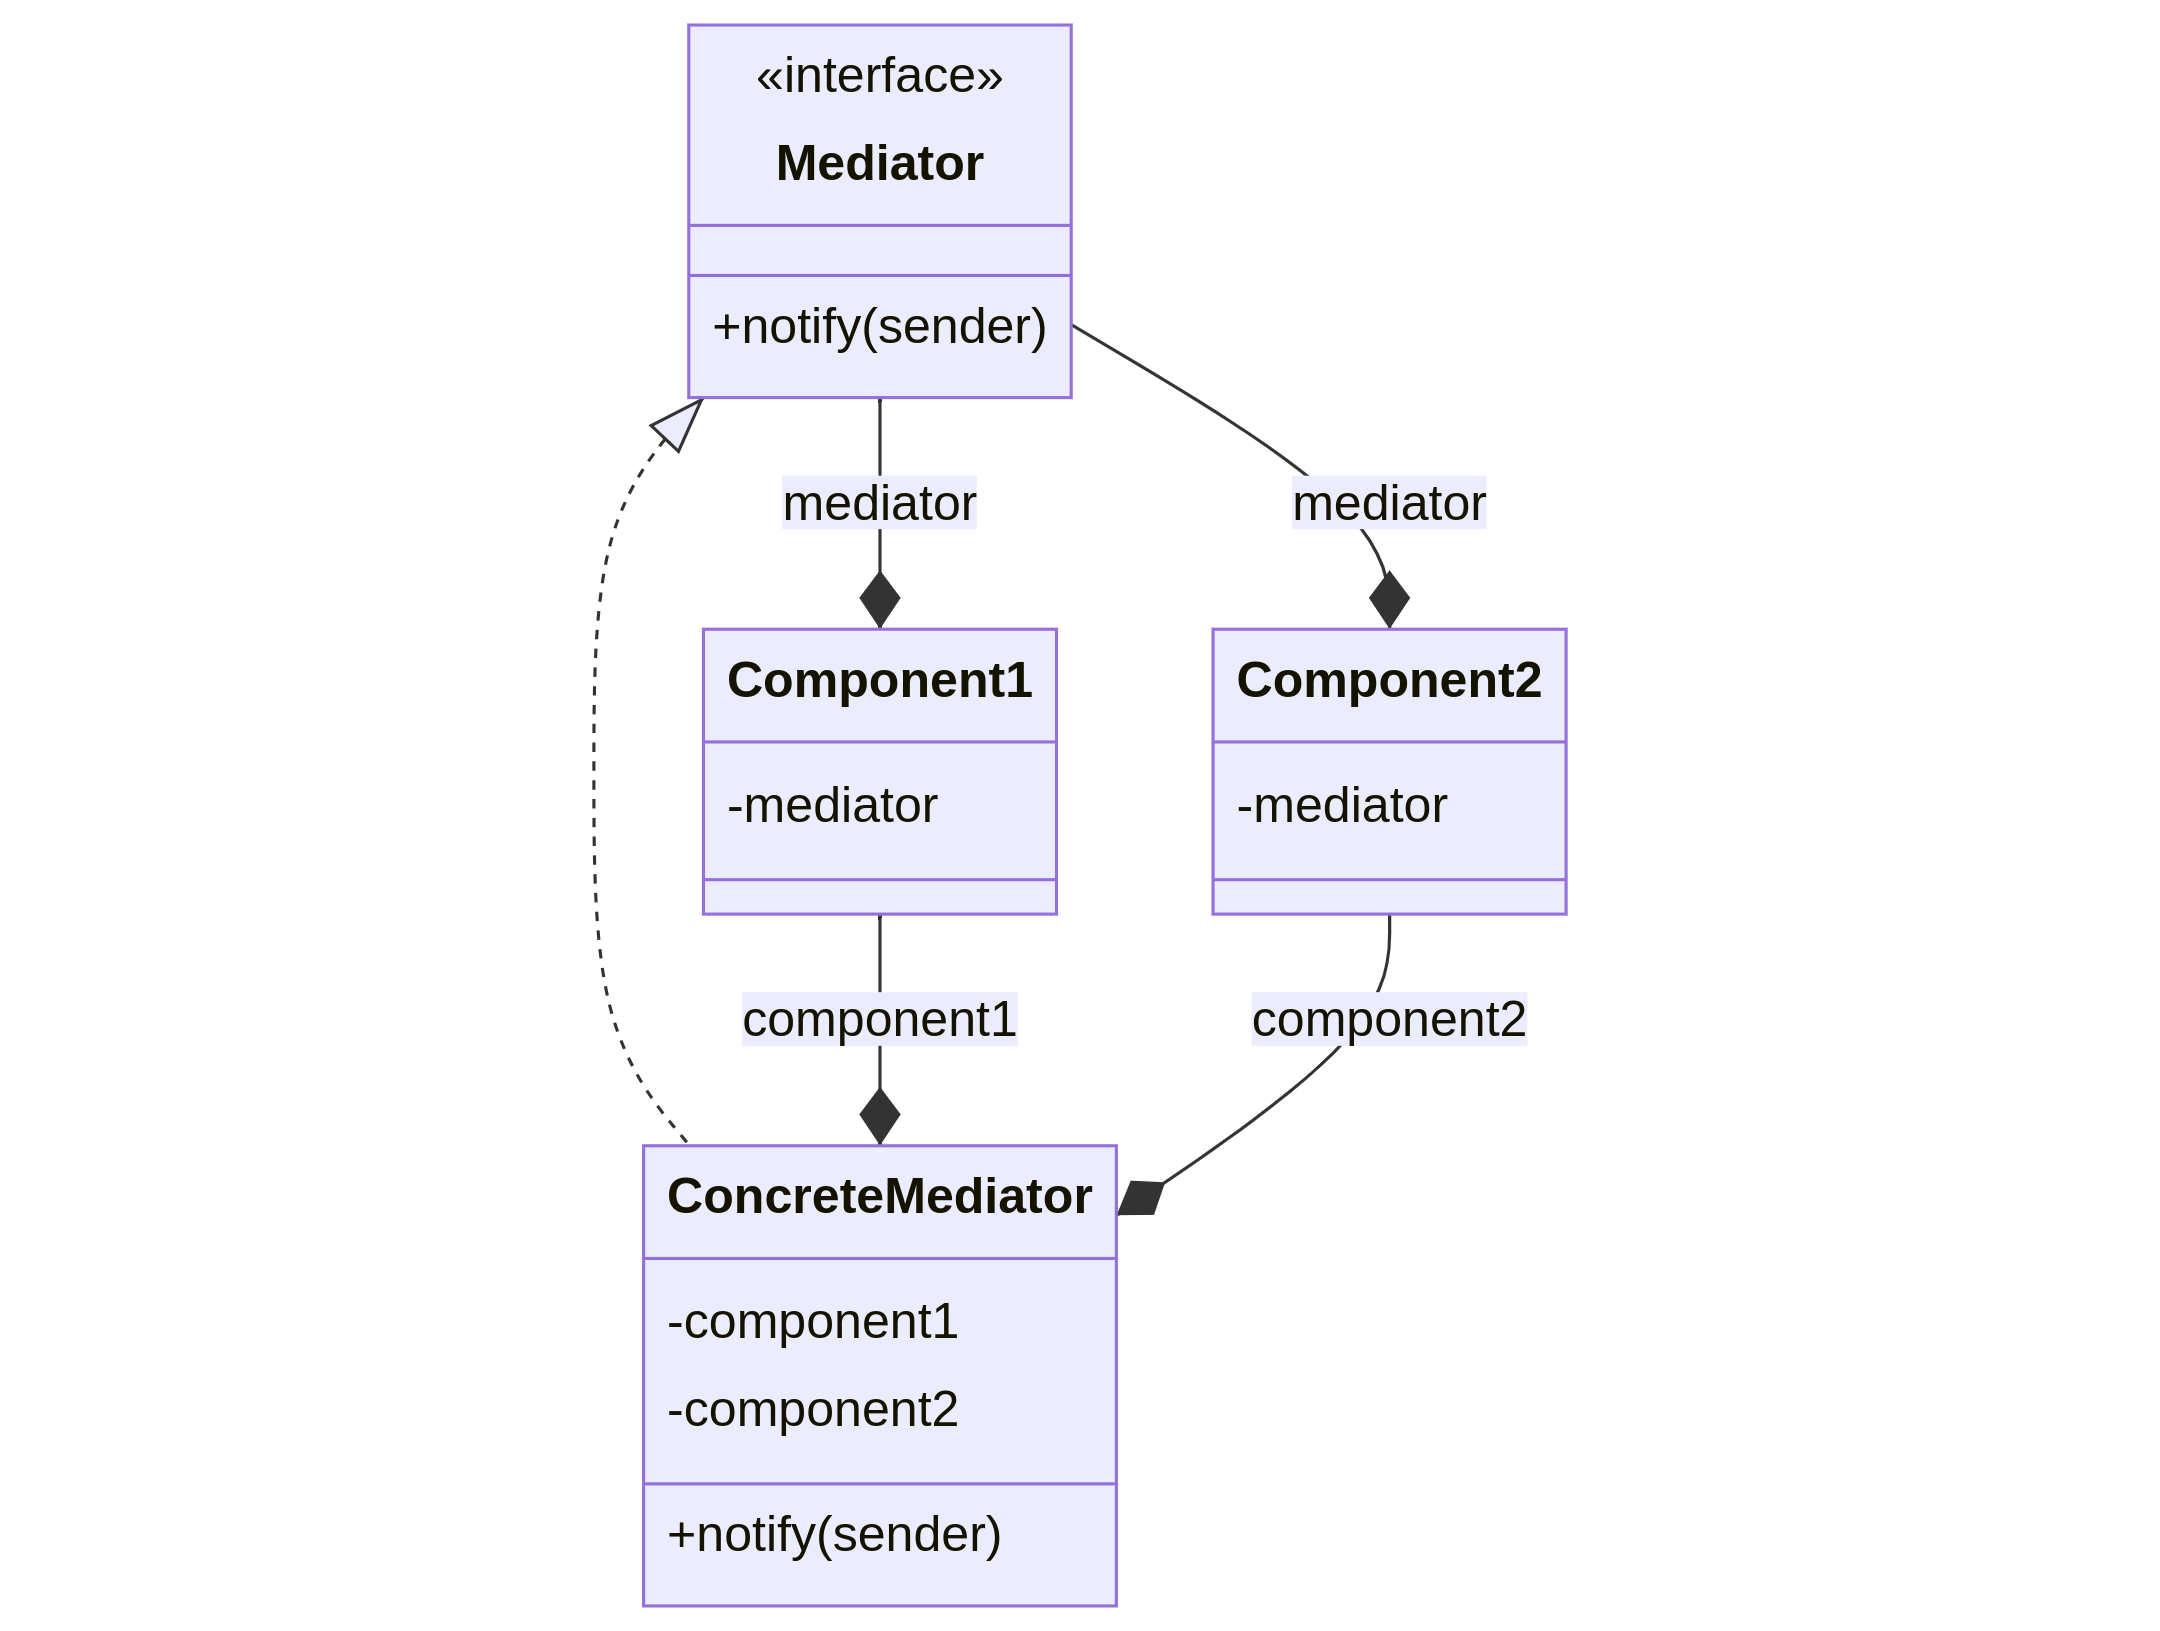
\includegraphics[width=0.75\linewidth]{images/patterns/mediator-class.png}
	\caption{Klassendiagramm Mediator Pattern}
	\label{fig:mediator-class}
\end{figure}

\subsubsection*{Konsequenzen}

Der Mediator kapselt Verhalten, welches ansonsten über mehrere Klassen verteilt wäre. Soll dieses Verhalten spezialisiert werden, so ist nur eine Spezialisierung des Mediators notwendig. Weiterhin verhindert der Mediator eine starke Kopplung der Komponenten. Komponenten- und Mediator-Klassen können bei kompatiblen Interfaces beliebig ausgetauscht werden. Der Mediator vereinfacht außerdem die Multiplizitäten von Objektinteraktionen. Er wandelt $m$:$n$- Beziehungen zwischen Objekten in $1$:$n$-Beziehungen zwischen den Objekten und dem Mediator um. 

Der Mediator bündelt Kontrolle an einem einzigen Punkt. Dies kann zur Übersichtlichkeit beitragen, kann dieser jedoch bei ausreichend komplexer Logik entgegenwirken. Das kann dem Mediator eine monolithische Struktur geben, deren Verhinderung seine eigentliche Aufgabe ist. 

Sind die Abhängigkeiten zwischen den Komponenten zu Komplex, so kann das Observer-Pattern zur Kommunikation zwischen den Komponenten und dem Mediator verwendet werden. Dadurch lassen sich die Abhängigkeiten außerdem flexibler gestalten, sie können also zur Laufzeit einfacher geändert werden.
\subsection{\emph{Visitor-Pattern} und \emph{Double Dispatch}}


\subsubsection*{Problembeschreibung}

Gelegentlich muss eine Operation auf einer Menge von Objekten durchgeführt, die alle Teil einer Objekthiearchie aber unterschiedlich sind. Diese Objekte besitzen daher unter Umständen voneinander abweichende Interfaces. Das \emph{Visitor-Pattern} erlaubt es, solche Operationen außerhalb der Objekte und für alle betroffenen Objekte innerhalb einer separaten Klasse zu definieren. \cite{gamma_design_1995}

\subsubsection*{Lösung}

Der konkrete \emph{Visitor}\footnote{Die deutsche Übersetzung ''Besucher'' ist in diesem Kontext eher unüblich.} (\code{ConcreteVisitor}) realisiert die \emph{Visitor}-Schnittstelle (\code{Visitor}), welche die Methode \code{visit} bereitstellt, wie in Abbildung \ref{fig:visitor-class} zu erkennen ist. Diese erlaubt es dem \emph{Visitor}, ein Element (\code{Element}) zu ''besuchen'' und auf ihm eine Operation durchzuführen. Die Elemente ''akzeptieren'' den ''Besuch'' des \emph{Visitors} mit Hilfe der Methode \code{accept}, welche als Argument den besuchenden\emph{Visitor} erhält.

\begin{figure}[H]
	\centering
	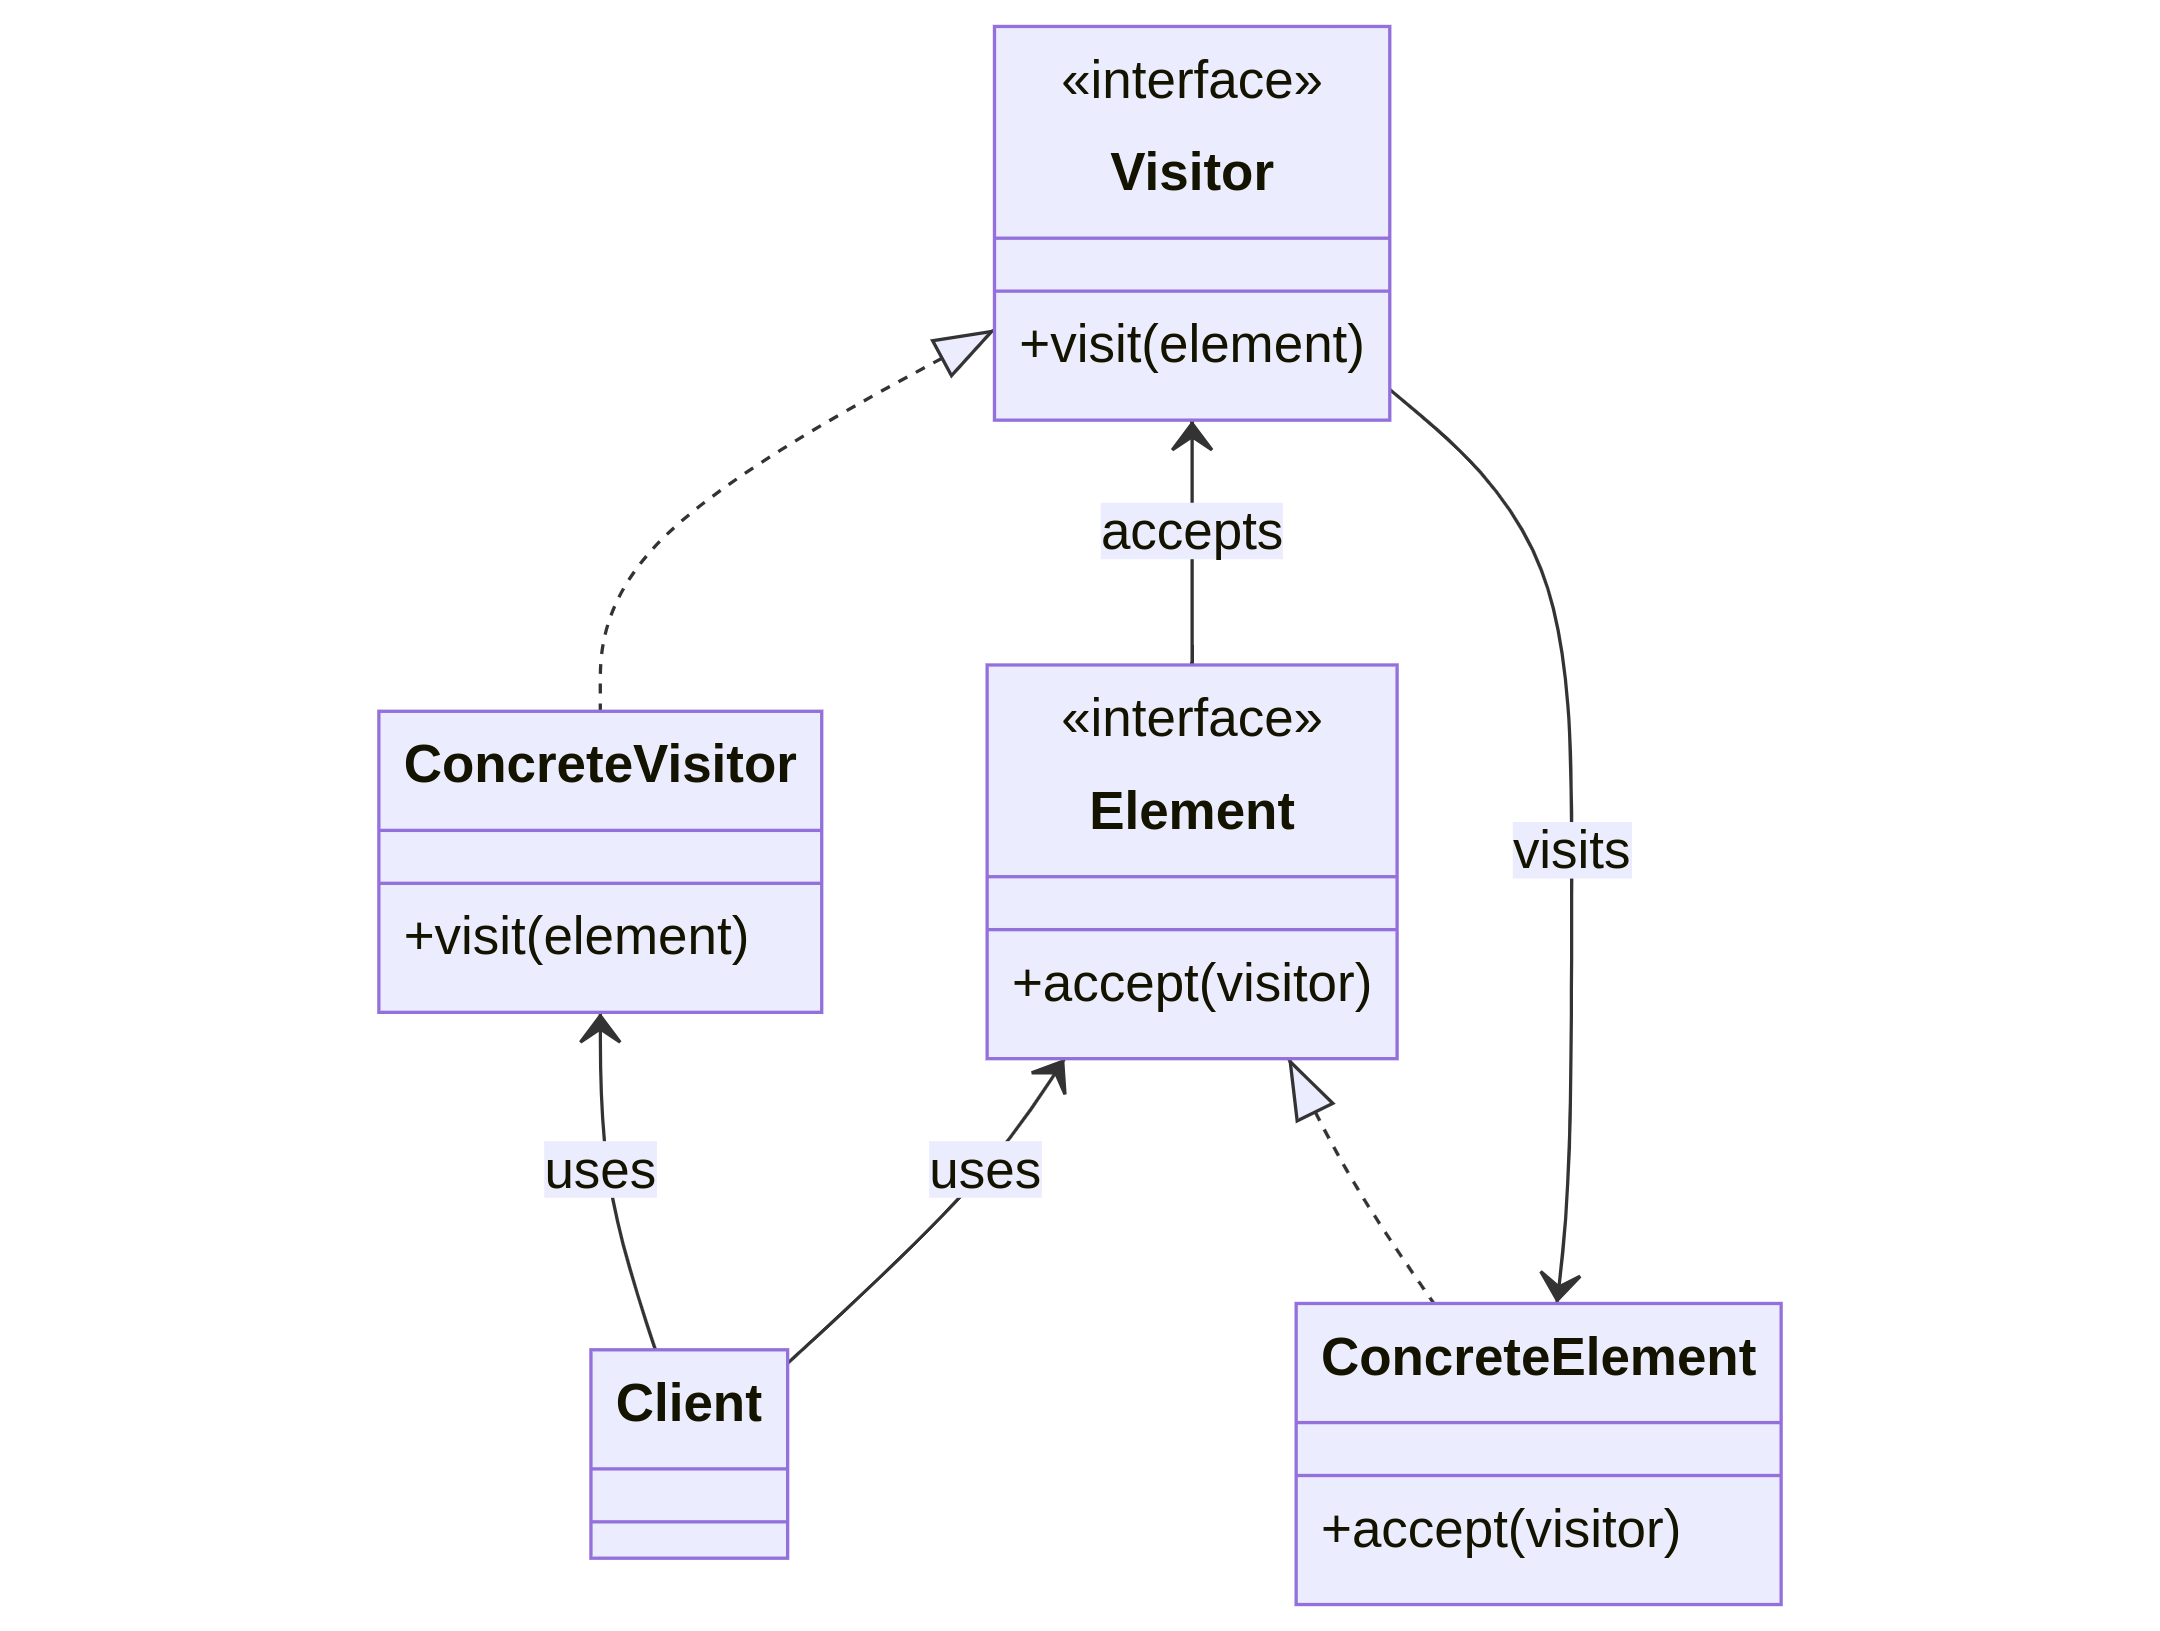
\includegraphics[width=0.75\linewidth]{images/patterns/visitor-class.png}
	\caption{Klassendiagramm des \emph{Visitor-Patterns}. \cite{skobeleva_visitor_2023}}
	\label{fig:visitor-class}
\end{figure}

Abbildung \ref{fig:visitor-seq} zeigt das Verhalten des \emph{Visitor-Patterns}. Der Anwender\footref{ftn:client} trägt dem\emph{Visitor} auf, eine Operation auf einem Element oder einer Menge von Elementen durchzuführen (1). Der\emph{Visitor} sendet daraufhin \code{visit} an alle Elemente, auf die er eine Referenz hält (2). Jedes Element ruft daraufhin eine \code{accept}-Methode auf dem\emph{Visitor} auf (3). Zu beachten ist hierbei, dass es für jede Element-Klasse eine eigene Methode im\emph{Visitor} gibt. Dies kann realisiert werden durch das Bereitstellen von Methoden mit unterschiedlichen, zu den aufrufenden Klassen korrespondierenden Namen oder durch Multimethoden. Multimethoden sind Methoden, welche je nach Typ der übergebenen Argumente unterschiedliche Implementierungen ausführen. Somit kann der\emph{Visitor} nach Erhalt von \code{accept} die zum Typ des sendenden Elements passende Operation ausführen. Dieser Mechanismus nennt sich \emph{Double-Dispatch}.

\begin{figure}[H]
	\centering
	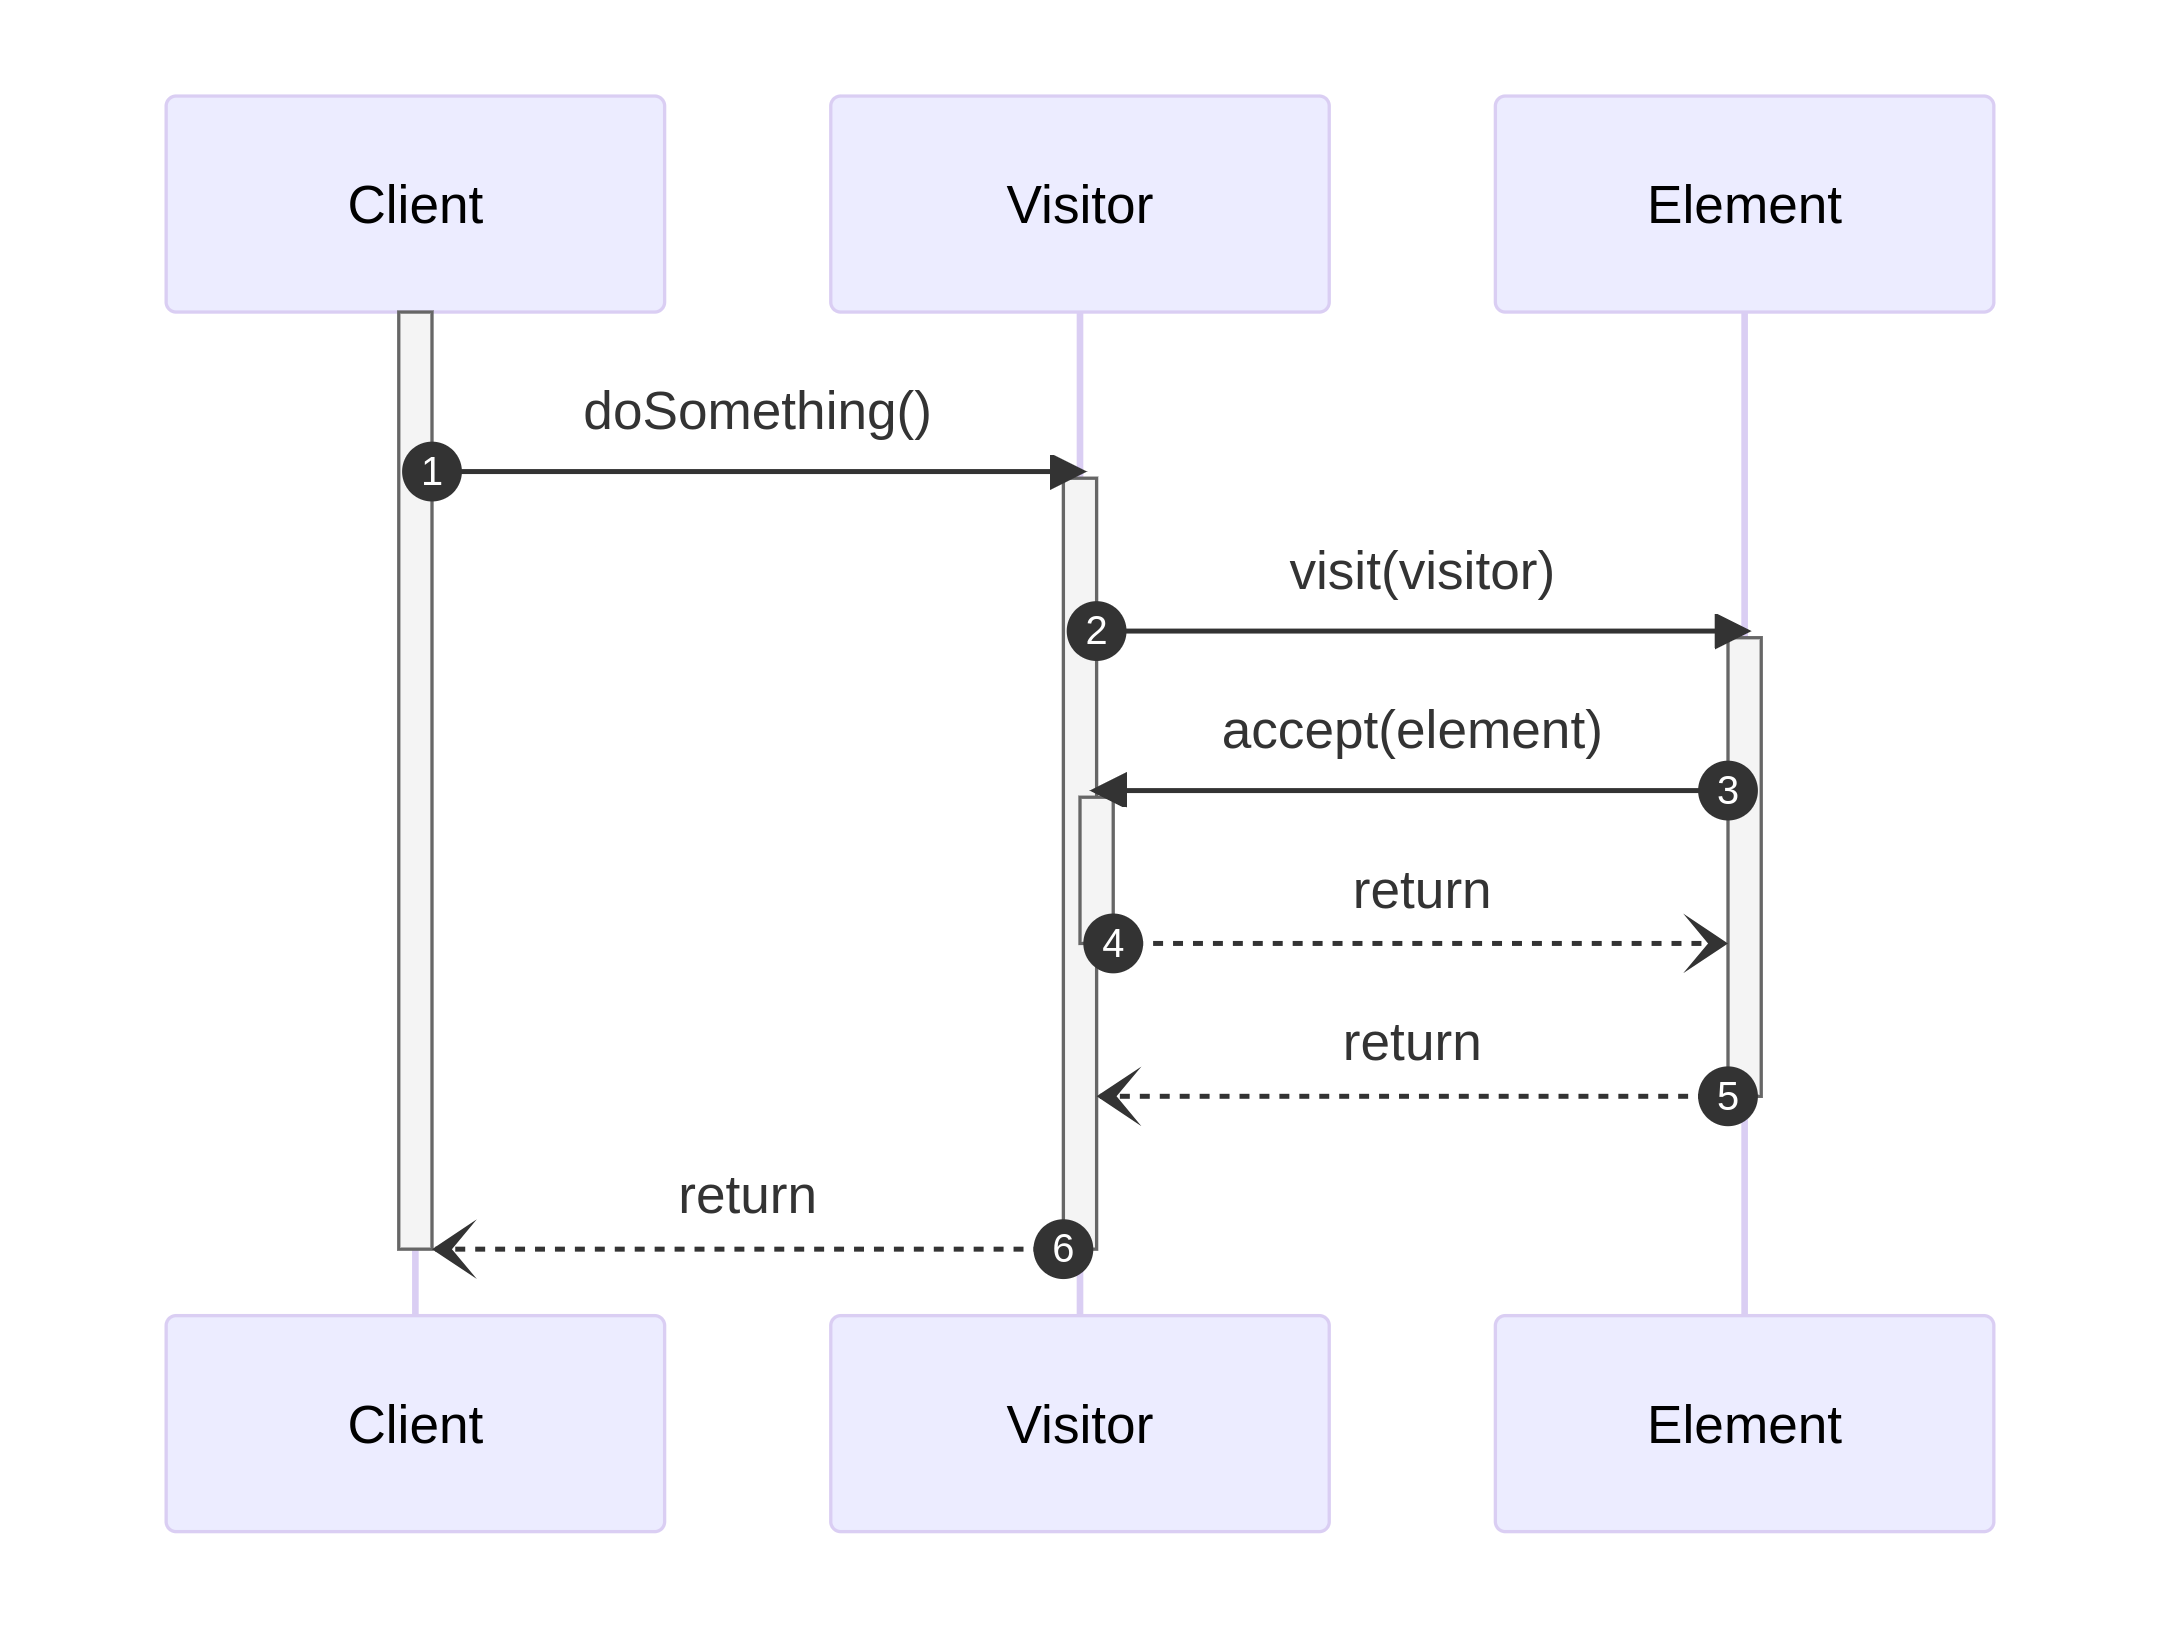
\includegraphics[width=0.75\linewidth]{images/patterns/visitor-seq.png}
	\caption{Sequenzdiagramm des \emph{Visitor-Patterns}. \cite{skobeleva_visitor_2023}}
	\label{fig:visitor-seq}
\end{figure}

\subsubsection*{Konsequenzen}
Durch die Kapselung der Operation in einem \emph{Visitor}, ist es sehr einfach, neue Operationen hinzuzufügen. Es bedarf dazu lediglich eines weiteren \emph{Visitors}. Außerdem kapselt ein\emph{Visitor} die Menge an Operationen auf den Elementen. Zusammengehörige Operationen werden in einer Klasse gesammelt. Nicht zueinander gehörende Operationen befinden sich in unterschiedlichen \emph{Visitors}. Ein weiterer Vorteil eines \emph{Visitors} ist dessen Fähigkeit, während des ''Besuchens'' mehrerer Elemente Informationen über diese zu akkumulieren und im Anschluss gebündelt zu repräsentieren.

Der\emph{Visitor}weist jedoch auch Nachteile auf. Zum einen ist es schwer, weitere konkrete Element-Klassen zu einem System hinzuzufügen, welches bereits eine Reihe an \emph{Visitors} besitzt. Da ein\emph{Visitor} für jeden Typ von Element eine Methode bereitstellen muss, kann ein weiteres Element einen erhöhten Implementierungsaufwand bedeuten. Das \emph{Visitor-Pattern} sollte daher nur verwendet werden, wenn entweder die Menge an Elementklassen abgeschlossen oder die Menge an \emph{Visitor}-Klassen übersichtlich ist. Weiterhin müssen die Elemente dem\emph{Visitor} eine Schnittstelle bereitstellen, welche es dem\emph{Visitor} ermöglicht, seine Operation ausführen zu können. Dies kann dazu führen, dass das Element einen großen Teil seines internen Zustands preisgeben muss, welcher bei nicht-Verwendung dieses Musters gekapselt geblieben wäre. \cite{gamma_design_1995}
\subsection{Factory Method}

\subsubsection*{Problembeschreibung}

Es wird eine Schnittstelle benötigt, um eine Reihe von Objekten erzeugen zu können. Jedes Objekt hat jedoch andere Anforderungen an seine Erzeugung. Eine \emph{Factory-Method} kann eingesetzt werden, wenn eine Klasse kein Wissen darüber besitzt oder besitzen soll, welches konkrete Objekt sie zu erzeugen hat oder wenn eine Klasse die Verantwortlichkeit über diese Entscheidung ihren Subklassen überlassen soll. \cite{gamma_design_1995}

\subsubsection*{Lösung}

Es existiert ein abstrakter Erzeuger (\code{Creator}), welcher eine Schnittstelle bereitstellt, um Produkte (\code{Product}) zu erzeugen. Die Details der Erzeugung dieser Produkte sind in den konkreten Subklassen der Erzeuger-Klasse implementiert. Jeder konkrete Erzeuger kann somit einen Typ von konkretem Produkt (\code{ConcreteProduct}) erschaffen. Das entsprechende Klassendiagramm ist in \autoref{fig:factory-method-class} dargestellt.

\begin{figure}[!ht]
	\centering
	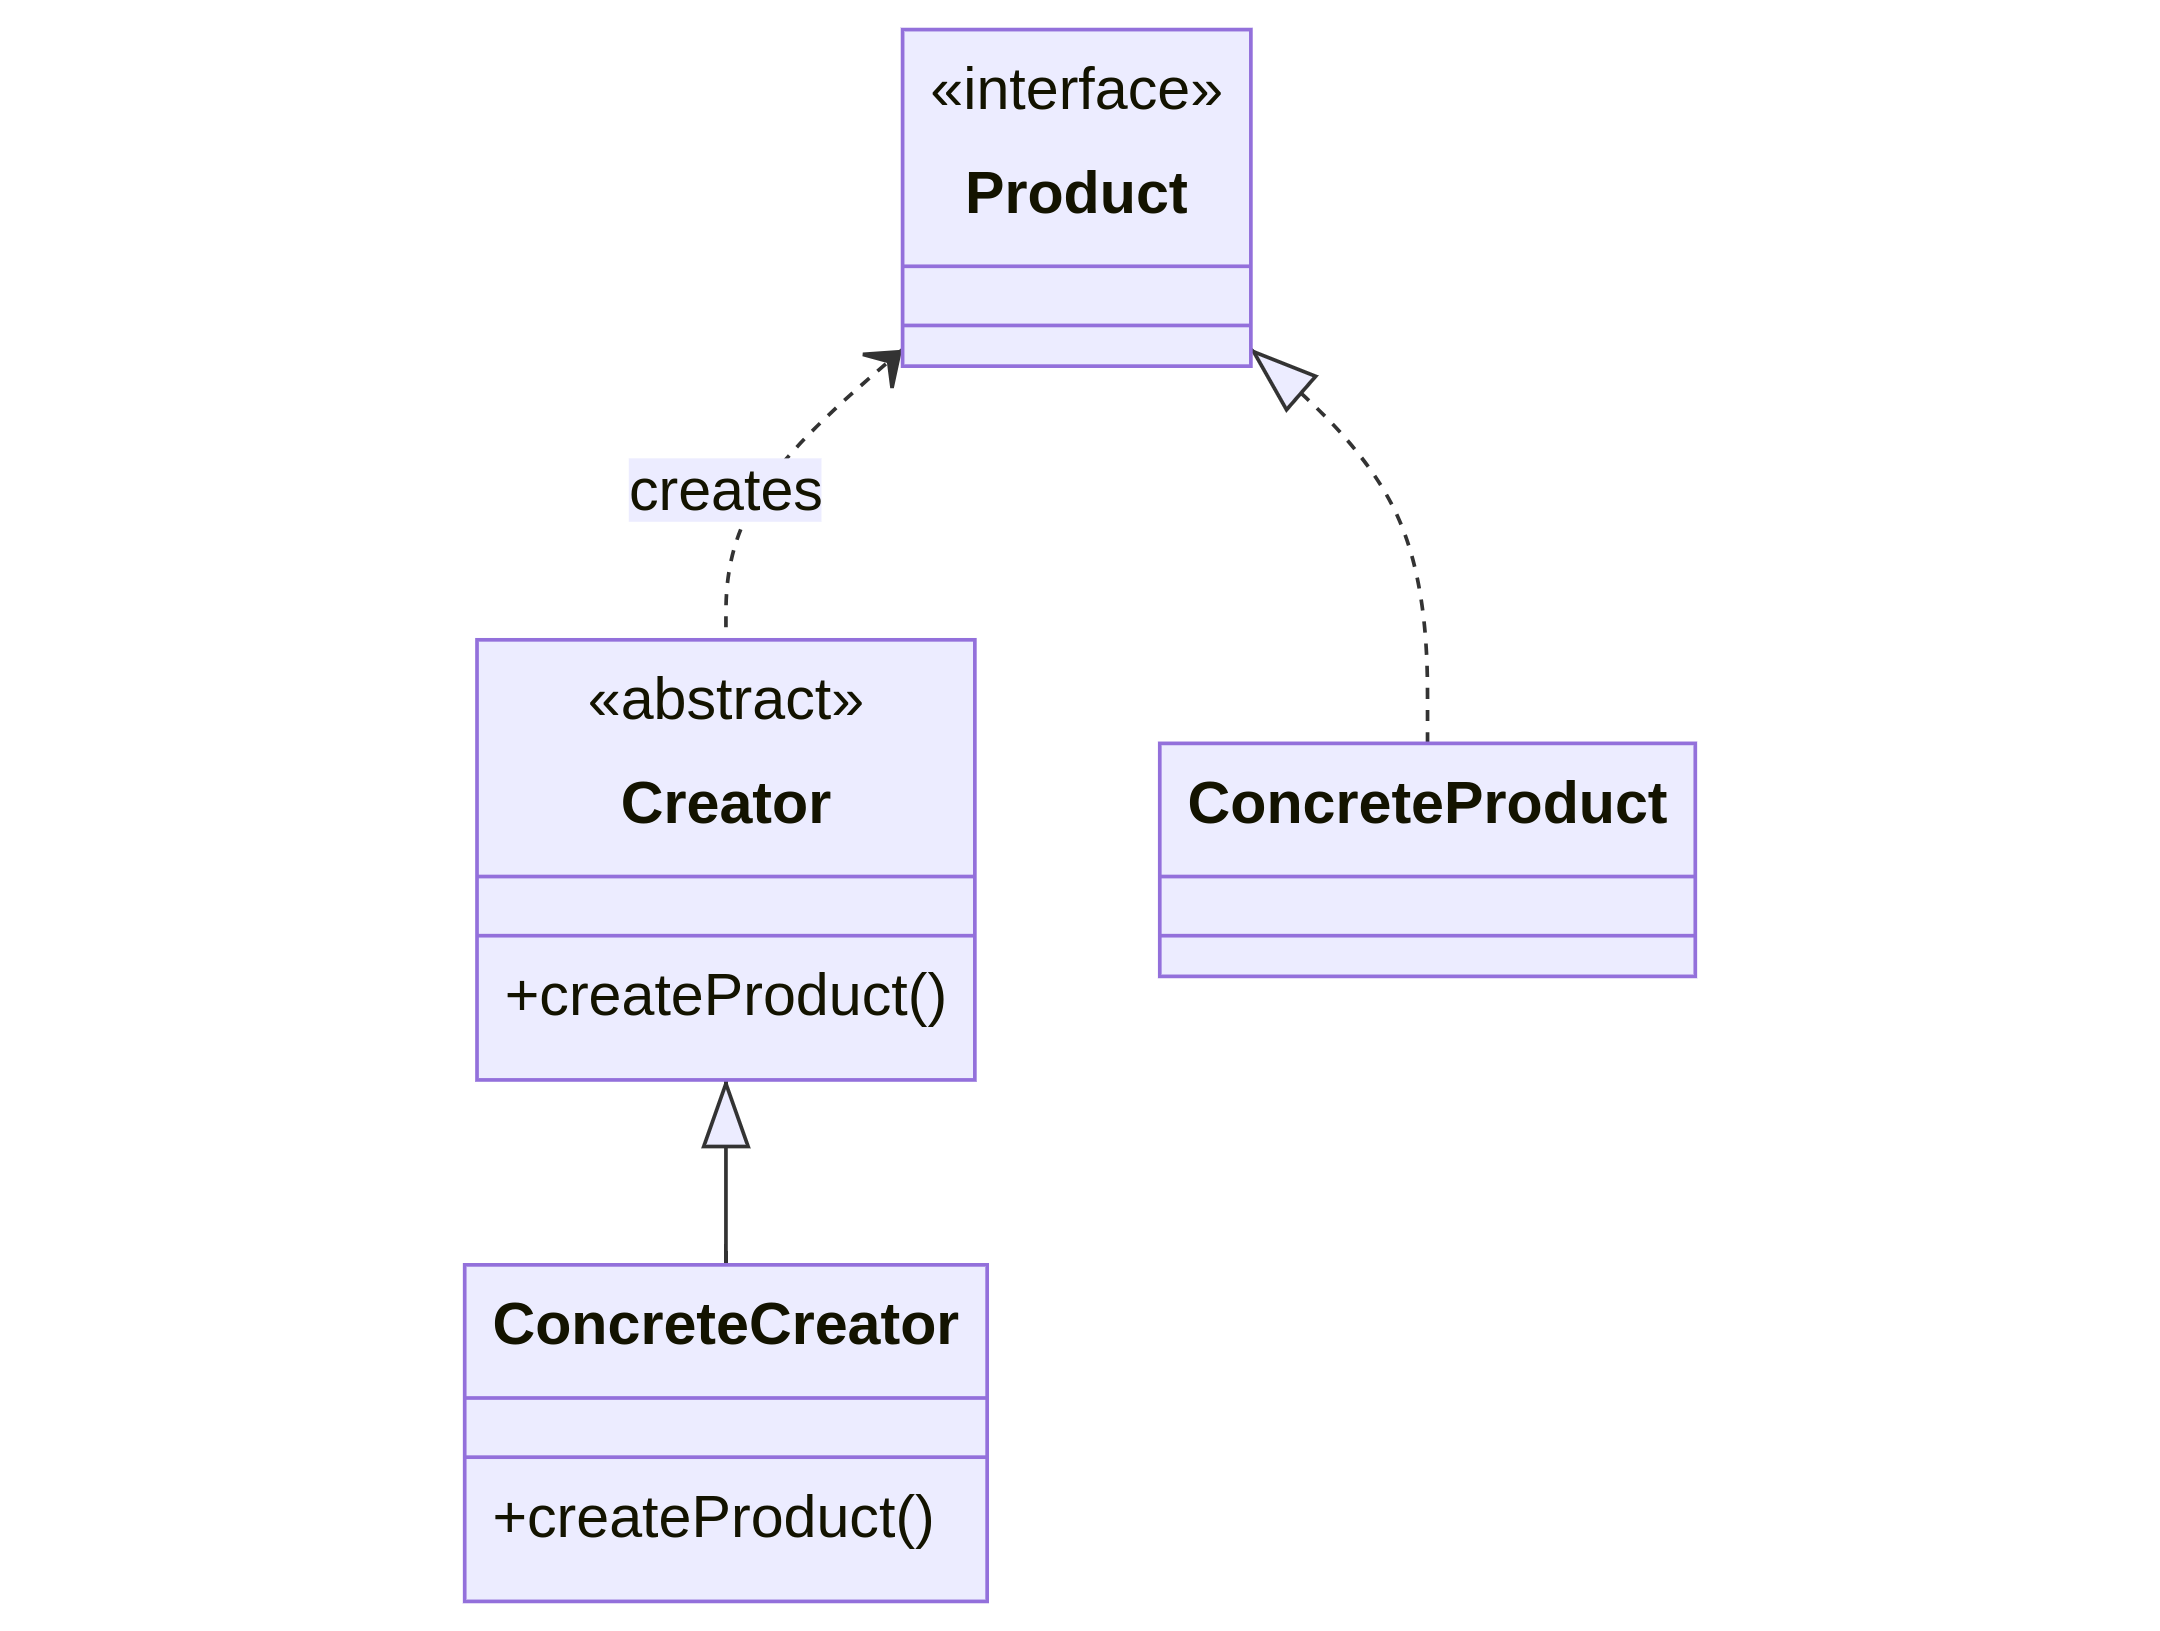
\includegraphics[width=0.75\linewidth]{images/patterns/factory-method-class.png}
	\caption{Klassendiagramm des \emph{Factory-Method}-Musters. Durch die Spiegelung der Vererbungshierarchie von Objekten entstehen Klassen, welche zur Erzeugung der Objekte verwendet werden können. \cite{skobeleva_factory_2023}}
	\label{fig:factory-method-class}
\end{figure}

\subsubsection*{Konsequenzen}
Ein Objekt über eine \emph{Factory-Method} zu erzeugen ist flexibler, als das Objekt direkt über den Konstruktor der Klasse zu instanziieren. Die erzeugende Klasse braucht nur das Interface des abstrakten Erzeugers zu kennen und ist somit in der Lage beliebige konkrete Produkte über deren korrespondierende konkrete Erzeuger zu instanziieren. Hierbei fällt auf, dass die Erzeuger-Klassenhierarchie die Produkt-Klassenhierarchie spiegelt. Für jeden Produkttyp existiert also auch eine Erzeuger-Klasse. Daraus kann sich jedoch auch ein Nachteil ergeben. Zur Nutzung eines Produktes müssen nun stets zwei Subklassen definiert und zur Laufzeit ein weiteres Objekt erstellt werden. Das erhöht die Komplexität. \cite{gamma_design_1995}

